\documentclass{beamer}\usepackage[]{graphicx}\usepackage[]{color}
%% maxwidth is the original width if it is less than linewidth
%% otherwise use linewidth (to make sure the graphics do not exceed the margin)
\makeatletter
\def\maxwidth{ %
  \ifdim\Gin@nat@width>\linewidth
    \linewidth
  \else
    \Gin@nat@width
  \fi
}
\makeatother

\definecolor{fgcolor}{rgb}{0.345, 0.345, 0.345}
\newcommand{\hlnum}[1]{\textcolor[rgb]{0.686,0.059,0.569}{#1}}%
\newcommand{\hlstr}[1]{\textcolor[rgb]{0.192,0.494,0.8}{#1}}%
\newcommand{\hlcom}[1]{\textcolor[rgb]{0.678,0.584,0.686}{\textit{#1}}}%
\newcommand{\hlopt}[1]{\textcolor[rgb]{0,0,0}{#1}}%
\newcommand{\hlstd}[1]{\textcolor[rgb]{0.345,0.345,0.345}{#1}}%
\newcommand{\hlkwa}[1]{\textcolor[rgb]{0.161,0.373,0.58}{\textbf{#1}}}%
\newcommand{\hlkwb}[1]{\textcolor[rgb]{0.69,0.353,0.396}{#1}}%
\newcommand{\hlkwc}[1]{\textcolor[rgb]{0.333,0.667,0.333}{#1}}%
\newcommand{\hlkwd}[1]{\textcolor[rgb]{0.737,0.353,0.396}{\textbf{#1}}}%
\let\hlipl\hlkwb

\usepackage{framed}
\makeatletter
\newenvironment{kframe}{%
 \def\at@end@of@kframe{}%
 \ifinner\ifhmode%
  \def\at@end@of@kframe{\end{minipage}}%
  \begin{minipage}{\columnwidth}%
 \fi\fi%
 \def\FrameCommand##1{\hskip\@totalleftmargin \hskip-\fboxsep
 \colorbox{shadecolor}{##1}\hskip-\fboxsep
     % There is no \\@totalrightmargin, so:
     \hskip-\linewidth \hskip-\@totalleftmargin \hskip\columnwidth}%
 \MakeFramed {\advance\hsize-\width
   \@totalleftmargin\z@ \linewidth\hsize
   \@setminipage}}%
 {\par\unskip\endMakeFramed%
 \at@end@of@kframe}
\makeatother

\definecolor{shadecolor}{rgb}{.97, .97, .97}
\definecolor{messagecolor}{rgb}{0, 0, 0}
\definecolor{warningcolor}{rgb}{1, 0, 1}
\definecolor{errorcolor}{rgb}{1, 0, 0}
\newenvironment{knitrout}{}{} % an empty environment to be redefined in TeX

\usepackage{alltt}
\usepackage{default}
\usepackage{animate} %need the animate.sty file 
\usepackage{graphicx}
%\graphicspath{{/home/sahir/Dropbox/jobs/laval/minicours/slides/}}
\usepackage{hyperref, url}
%\usepackage[round,sort]{natbib}   % bibliography omit 'round' option if you prefer square brackets
%\bibliographystyle{apalike}
\usepackage{biblatex}
\bibliography{bib.bib}
% Removes icon in bibliography
\setbeamertemplate{bibliography item}[text]

\usepackage[normalem]{ulem}

\setbeamertemplate{theorems}[numbered]
\usepackage[final]{pdfpages}



%\newtheorem{prop}{Proposition}
%\newenvironment{theoremc}[1]
%{\begin{shaded}\begin{theorem}[#1]}
%		{\end{theorem}\end{shaded}}

%\newtheorem{examplefirst}{Example}
%\newtheorem{examplesecond}{Example}
%\newenvironment<>{examplefirst}[1][]{%
%	\setbeamercolor{block title example}{bg=lightgray}%
%	\begin{example}#2[#1]}{\end{example}}
%\newenvironment<>{examplesecond}[1][]{%
%	\setbeamercolor{block title example}{fg=white,bg=blue!75!black}%
%	\begin{example}#2[#1]}{\end{example}}	

%\usepackage{amsthm}


\usepackage[figurename=Fig.]{caption}
\usepackage{subfig}
\usepackage{tikz, pgfplots,epsfig}
\usetikzlibrary{arrows,shapes.geometric}
\usepackage{color, colortbl,xcolor}
\definecolor{lightgray}{RGB}{200,200,200}
\definecolor{palegray}{RGB}{221,221,221}
\definecolor{myblue}{RGB}{0,89,179}
\usepackage{comment}
\setbeamercolor{frametitle}{fg=myblue}
\setbeamercolor{section in head/foot}{bg=myblue, fg=white}
\setbeamercolor{author in head/foot}{bg=myblue}
\setbeamercolor{date in head/foot}{bg=myblue}

\usepackage{shadethm}
%\colorlet{shadecolor}{blue!15}
\colorlet{shadecolor}{palegray}
%\setlength{\shadeboxrule}{.4pt}

\newshadetheorem{thm}{Theorem}
\newshadetheorem{defm}{Definition}
\newshadetheorem{exm}{Exercise}
\newshadetheorem{remarkm}{Remark}
%\definecolor{shadethmcolor}{HTML}{EDF8FF}
\definecolor{shadethmcolor}{RGB}{221,221,221}
%\definecolor{shaderulecolor}{HTML}{45CFFF}
\definecolor{shaderulecolor}{RGB}{0,89,179}
\setlength{\shadeboxrule}{.4pt}


\usepackage{array}
\newcolumntype{L}{>{\centering\arraybackslash}m{3cm}} % used for text wrapping in ctable
\usepackage{ctable}
\usepackage[utf8]{inputenc}
\usepackage{fontenc}
\usepackage{pifont}% http://ctan.org/pkg/pifont
\newcommand{\cmark}{\ding{51}}%
\newcommand{\xmark}{\ding{55}}%
\def\widebar#1{\overline{#1}}
\definecolor{whitesmoke}{rgb}{0.96, 0.96, 0.96}

\usepackage{amssymb}
\usepackage{amsmath}

\usepackage{bm}
\def\transpose{{\sf{T}}}
\def\E{{\skew0\bm{E}}}
\def\Xvec{{\skew0\bm{X}}}
\def\Xveca{{\skew0\bm{X}}_1}
\def\Xvecb{{\skew0\bm{X}}_2}

\def\Yvec{{\skew0\bm{Y}}}
\def\bmY{{\skew0\bm{Y}}}
\def\bmX{{\skew0\bm{X}}}
\def\bmy{{\skew0\bm{y}}}
\def\bmG{{\skew0\bm{G}}}
\def\bmS{{\skew0\bm{S}}}
\def\bmA{{\skew0\bm{A}}}
\def\bmB{{\skew0\bm{B}}}
\def\bmD{{\skew0\bm{D}}}
\def\bmI{{\skew0\bm{I}}}
\def\bmV{{\skew0\bm{V}}}
\def\bmU{{\skew0\bm{U}}}
\def\bv{{\skew0\bm{v}}}
\def\bw{{\skew0\bm{w}}}
\def\bmm{{\skew0\bm{m}}}
\def\bmzero{{\skew0\bm{0}}}
\def\bx{{\skew0\bm{x}}}
\def\xveca{{\skew0\bm{x}}_1}
\def\xvecb{{\skew0\bm{x}}_2}

\def\N{{\skew0\mathcal{N}}}
\def\T{{\small T}}

\def\mvec{{\skew0\bm{m}}}
\def\bmmu{{\skew0\bm{\mu}}}
\def\muvec{{\skew0\bm{\mu}}}
\def\balpha{{\skew0\bm{\alpha}}}
\def\bbeta{{\skew0\bm{\beta}}}
\def\bmtheta{{\skew0\bm{\theta}}}
\def\btheta{{\skew0\bm{\theta}}}

\def\cvec{{\skew0\mathbf{c}}}

\def\Xbar{\overline{X}}

\definecolor{lightgray}{rgb}{0.91,0.91,0.91}
\definecolor{purpleblue}{rgb}{0.50,0.50,1.00}



\usepackage{fontspec}
%\setsansfont{Fira Sans}
%\setmonofont{Fira Mono}
\setsansfont[ItalicFont={Fira Sans Light Italic},BoldFont={Fira Sans},BoldItalicFont={Fira Sans Italic}]{Fira Sans Light}
\setmonofont[BoldFont={Fira Mono Medium}]{Fira Mono}


\setbeamercolor{itemize item}{fg=myblue}
\setbeamertemplate{itemize item}[square]

\setbeamertemplate{navigation symbols}{\usebeamercolor[fg]{title in head/foot}\usebeamerfont{title in head/foot}\insertframenumber}
\setbeamertemplate{footline}{}

\newtheorem{proposition}[theorem]{Proposition}
\newtheorem{exercise}[theorem]{Exercise}

\titlegraphic{\hfill
\includegraphics[height=1cm]{mcgill_logo.png}}


%% You also use hyperref, and pick colors 
\hypersetup{colorlinks,citecolor=orange,filecolor=red,linkcolor=brown,urlcolor=blue}

\newcommand {\framedgraphiccaption}[2] {
	\begin{figure}
		\centering
		\includegraphics[width=\textwidth,height=0.8\textheight,keepaspectratio]{#1}
		\caption{#2}
	\end{figure}
}

\newcommand {\framedgraphic}[1] {
	\begin{figure}
		\centering
		\includegraphics[width=\textwidth,height=0.9\textheight,keepaspectratio]{#1}
	\end{figure}
}


\AtBeginSection[]{
	\begin{frame}
	\vfill
	\centering
	\begin{beamercolorbox}[sep=8pt,center,shadow=true,rounded=true]{title}
		\usebeamerfont{title}\insertsectionhead\par%
	\end{beamercolorbox}
	\vfill
\end{frame}
}

\newcommand\Wider[2][3em]{%
\makebox[\linewidth][c]{%
	\begin{minipage}{\dimexpr\textwidth+#1\relax}
		\raggedright#2
	\end{minipage}%
}%
}



\newcommand{\blue}[1]{\textcolor{blue}{#1}}
\newcommand{\red}[1]{\textcolor{red}{#1}}
%\makeatother

\usepackage{xparse}
\NewDocumentCommand\mylist{>{\SplitList{;}}m}
{
\begin{itemize}
	\ProcessList{#1}{ \insertitem }
\end{itemize}
}
\NewDocumentCommand\mynum{>{\SplitList{;}}m}
{
\begin{enumerate}
	\ProcessList{#1}{ \insertitem }
\end{enumerate}
}
\newcommand\insertitem[1]{\item #1}

\newcommand\FrameText[1]{%
\begin{textblock*}{\paperwidth}(0pt,\textheight)
	\raggedright #1\hspace{.5em}
\end{textblock*}}
\IfFileExists{upquote.sty}{\usepackage{upquote}}{}
\begin{document}
%\sffamily



%\title{Introduction to Regression Trees}
%\author{Sahir Bhatnagar \inst{1}}
%\author[shortname]{Sahir Rai Bhatnagar, PhD Candidate (Biostatistics) }
%\institute[shortinst]{Department of Epidemiology, Biostatistics and Occupational Health}

\title{Logistic Regression}
%\subtitle{\href{https://www.dropbox.com/s/1l3i59rw1qsnmsz/EPIB607introToRegression.pdf?dl=0}{JH notes on regression}}
\author{Sahir Bhatnagar and James Hanley}
\institute{
	EPIB 607\\
	Department of Epidemiology, Biostatistics, and Occupational Health\\
	McGill University\\
	
	\vspace{0.1 in}
	
	\texttt{sahir.bhatnagar@mcgill.ca}\\
	\texttt{\url{https://sahirbhatnagar.com/EPIB607/}}}

%\date

\maketitle

\section{Parameter-contrasts}

\begin{frame}{Introduction to parameter-contrasts}

\begin{itemize}
	\setlength\itemsep{2em}
	\item We started the course by talking about the case where there were no determinants, i.e., no subpopulations $\to$ there was one global parameter ($\mu$, $\pi$, $\lambda$). \pause 
	\item Now we concern ourselves with determinants of the global parameter. For example:
	\begin{itemize}
		\item $\mu_{north}$ vs. $\mu_{south}$
		\item $\pi_{north}$ vs. $\pi_{south}$
		\item $\lambda_{north}$ vs. $\lambda_{south}$
	\end{itemize}
	\pause 
	\item Today we introduce population parameter \underline{contrasts} in a regression framework
	
\end{itemize}

\end{frame}

\begin{frame}
\Wider[8em]{
	\centering
	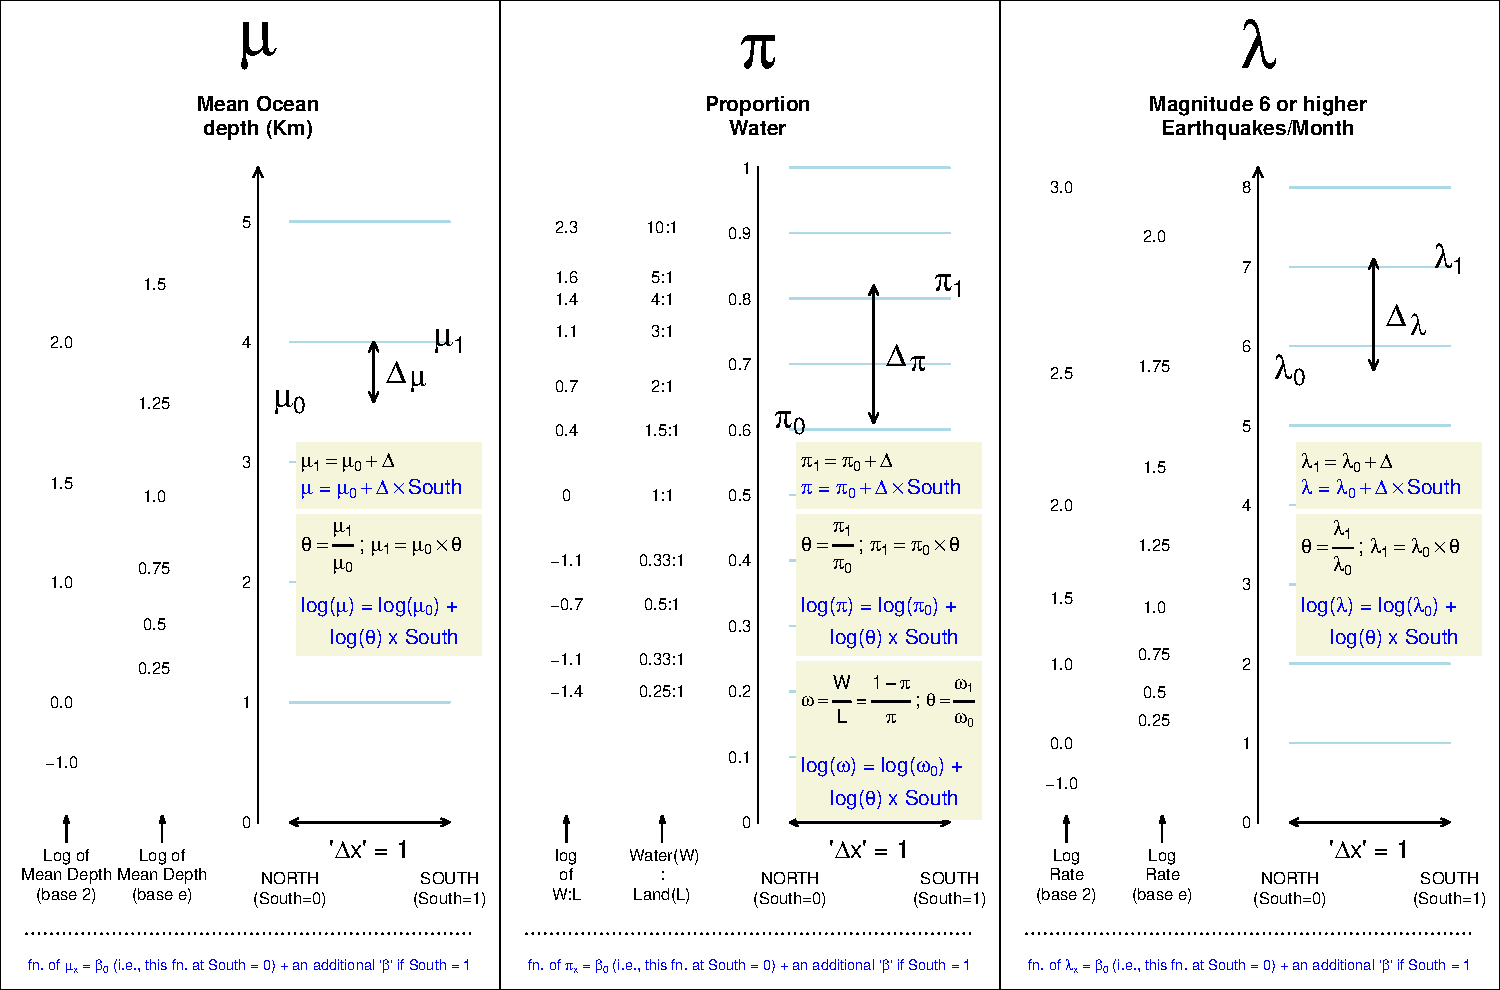
\includegraphics[width=4.9in,height=3.6in]{Fig16.pdf}
}
\end{frame}

\end{document}


%%%%%%%%%%%%%%%%%%%%%%%%%%%%%%%%%%%%%%%%%%%%%%%%%%%%%%%%%%%%%%%%%%%%%%%%%%%%%%%%%%%%%%%%%%%%%%%%%%%%%%%%%%%%%%%%%%%%%%%
%%%%%%%%%%%%%%%%%%%%%%%%%%%%%%%%%%%%%%%%%%%%%%%%%%%%%%%%%%%%%%%%%%%%%%%%%%%%%%%%%%%%%%%%%%%%%%%%%%%%%%%%%%%%%%%%%%%%%%%
%%%%%%%%%%%%%%%%%%%%%%%%%%%%%%%%%%%%%%%%%%%%%%%%%%%%%%%%%%%%%%%%%%%%%%%%%%%%%%%%%%%%%%%%%%%%%%%%%%%%%%%%%%%%%%%%%%%%%%%
%%%%%%%%%%%%%%%%%%%%%%%%%%%%%%%%%%%%%%%%%%%%%%%%%%%%%%%%%%%%%%%%%%%%%%%%%%%%%%%%%%%%%%%%%%%%%%%%%%%%%%%%%%%%%%%%%%%%%%%
%%%%%%%%%%%%%%%%%%%%%%%%%%%%%%%%%%%%%%%%%%%%%%%%%%%%%%%%%%%%%%%%%%%%%%%%%%%%%%%%%%%%%%%%%%%%%%%%%%%%%%%%%%%%%%%%%%%%%%%
%%%%%%%%%%%%%%%%%%%%%%%%%%%%%%%%%%%%%%%%%%%%%%%%%%%%%%%%%%%%%%%%%%%%%%%%%%%%%%%%%%%%%%%%%%%%%%%%%%%%%%%%%%%%%%%%%%%%%%%


\begin{frame}{Why regression for parameter-contrasts?}

\begin{itemize}
	\setlength\itemsep{1.5em}
\item Why do we start in a regression framework (as opposed to two-sample inference in B\&M and AAO)? \pause 
\item \textbf{Parameter contrasts are a special case of regression} \pause 
\item Approach taken in Miettinen, Clayton in Hills, Rothman and Greenland, baby Rothman
\end{itemize}

\end{frame}


\begin{frame}{What is regression?}

\begin{itemize}
	\setlength\itemsep{2em}
\item How \textbf{parameters} relate to its determinants \pause
\item How to link the parameters between the different populations through generic equations, that looks like a regression equation. \pause 
\item Then once you get data, you can actually fit or get your best estimates of those parameters
\end{itemize}

\end{frame}

\begin{frame}{Linear regression: The Concept}

\begin{itemize}
	\setlength\itemsep{2em}
	\item A regression model is said to be \textbf{linear} when it is of the form 
	\begin{align*}
	\mu & = \mu_0 + \sum_{j=1}^p \beta_j X_j \\
	& = \mu_0 + \beta_1 X_1 +  \beta_1 X_1 + \cdots +  \beta_p X_p
	\end{align*}
	
	\item Which means that the value of the mean ($\mu$) is viewed as a linear combination of the parameters $\mu_0, \beta_1, \beta_2, \ldots, \beta_p$, the coefficients of the linear combination being the realizations for the $X$'s

\end{itemize}

\end{frame}

\begin{frame}{Linear regression: Example}

\begin{itemize}
	\setlength\itemsep{2em}
	\item Consider intraoperative mortality in open-heart surgery. 
	\item Here, $\mu$ designates the incidence (risk) of intraoperative death. \pause 
	\item For this parameter of occurrence one might consider the determinants 
	\begin{itemize}
		\item $X_1$: congestive heart failure (CHF), represented by an indicator variable
		
$$
X_1 = \begin{cases}
1 & \textrm{if CHF}\\
0 & \textrm{otherwise}
\end{cases}
$$
		\pause
		\item $X_2$: duration of cardiac bypass in minutes
	\end{itemize} 
	
\end{itemize}

\end{frame}



\begin{frame}{Linear regression: Example}

\begin{itemize}
	\setlength\itemsep{1.7em}
	\item The model might be taken as 
$$
\mu = \mu_0 + \beta_1 X_1 + \beta_2 X_2
$$

and provides the average risk among population members of a \underline{given} $X_1$ and $X_2$

\item An individual's risk $\mu$ is a linear combination of $\mu_0, \beta_1$ and $\beta_2$


\pause 

\item If we had an infinite amount of data, an individual's risk would be determined by their CHF status and the duration of cardiac bypass:

$$
\mu = \begin{cases}
\mu_0 + \beta_1 + \beta_2 X_2 &  \textrm{if CHF}\\
\mu_0 + \beta_2 X_2 &  \textrm{otherwise}
\end{cases}
$$
	
\end{itemize}

\end{frame}




\section{Regression equations when the truth is known}

\begin{frame}
\Wider[8em]{
	\centering
	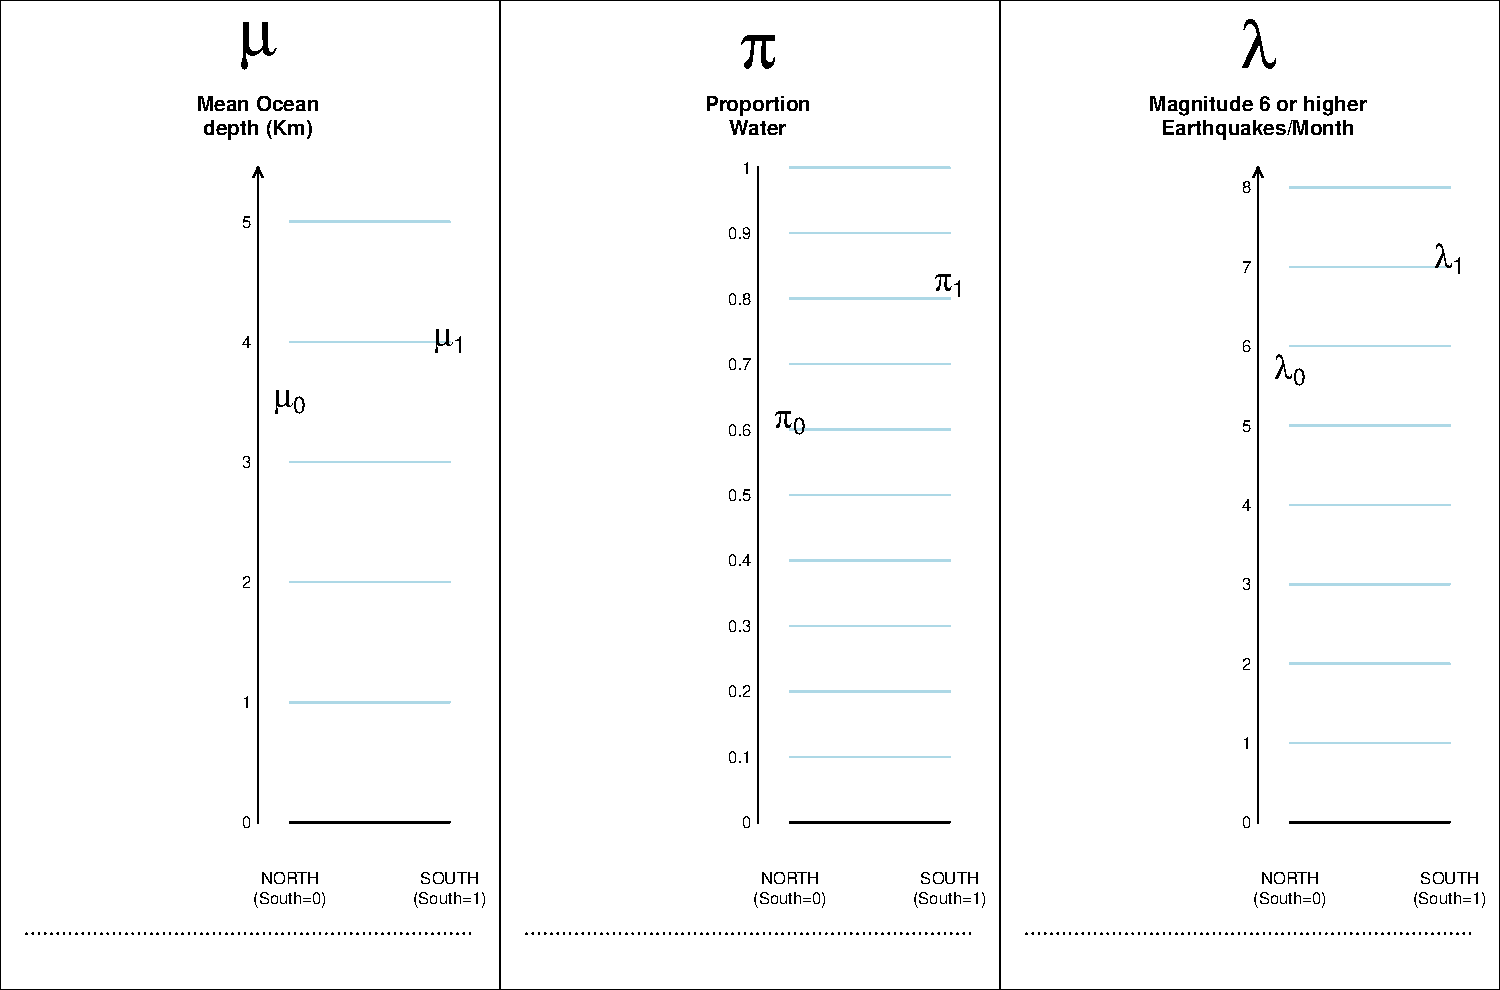
\includegraphics[width=4.9in,height=3.6in]{Fig10.pdf}
}
\end{frame}

\begin{frame}
\Wider[8em]{
	\centering
	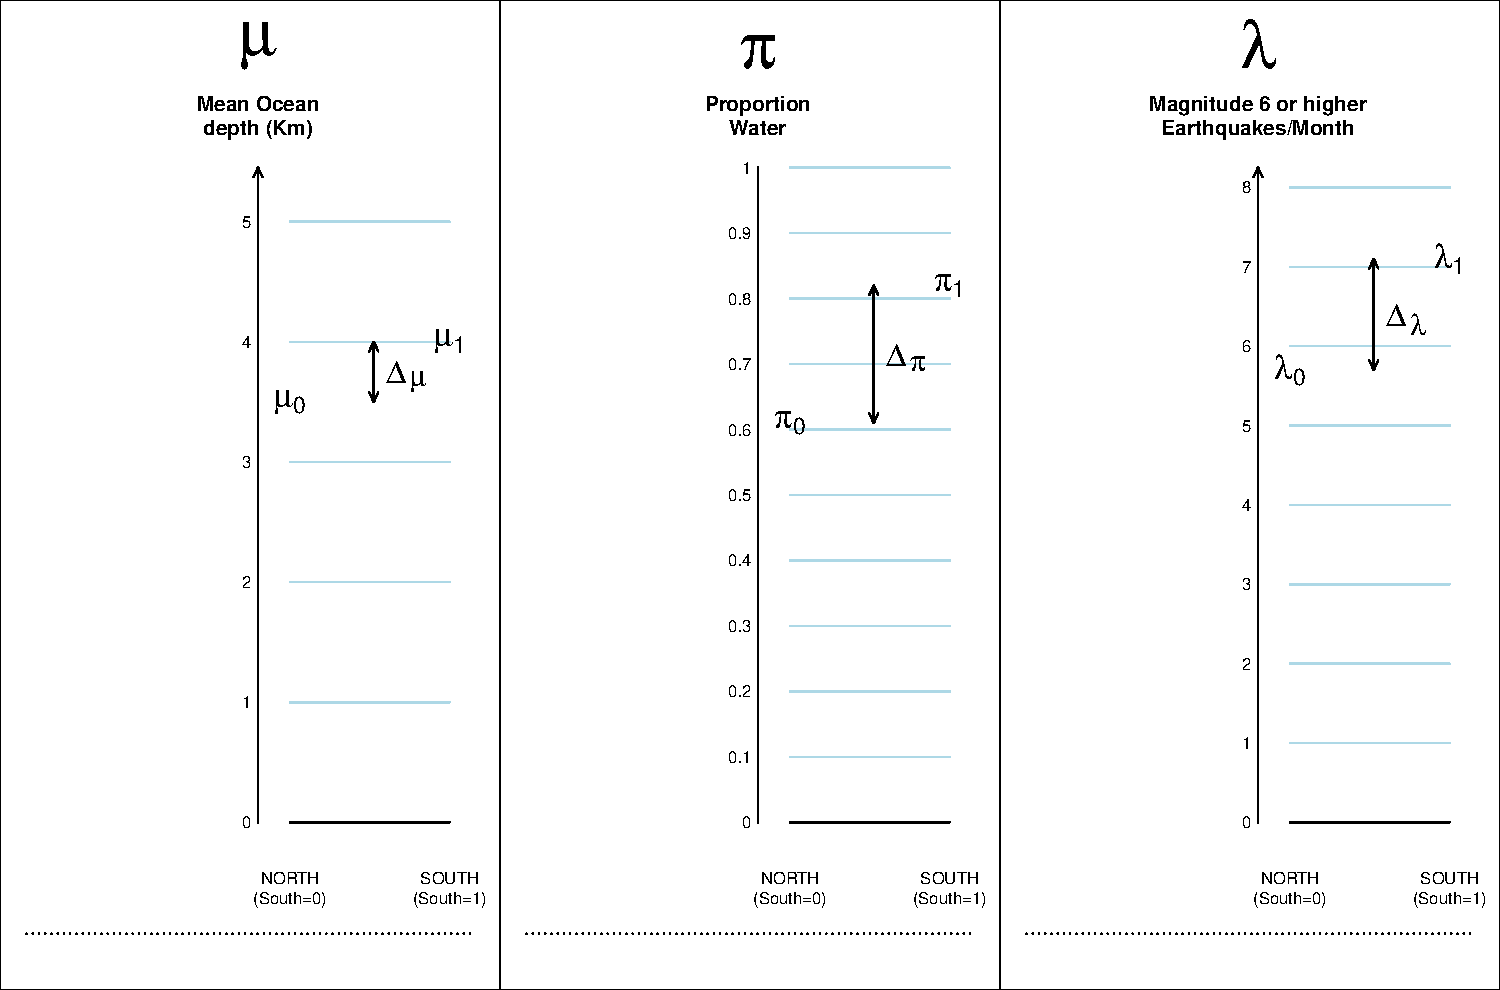
\includegraphics[width=4.9in,height=3.6in]{Fig11.pdf}
}
\end{frame}


\begin{frame}
\Wider[8em]{
	\centering
	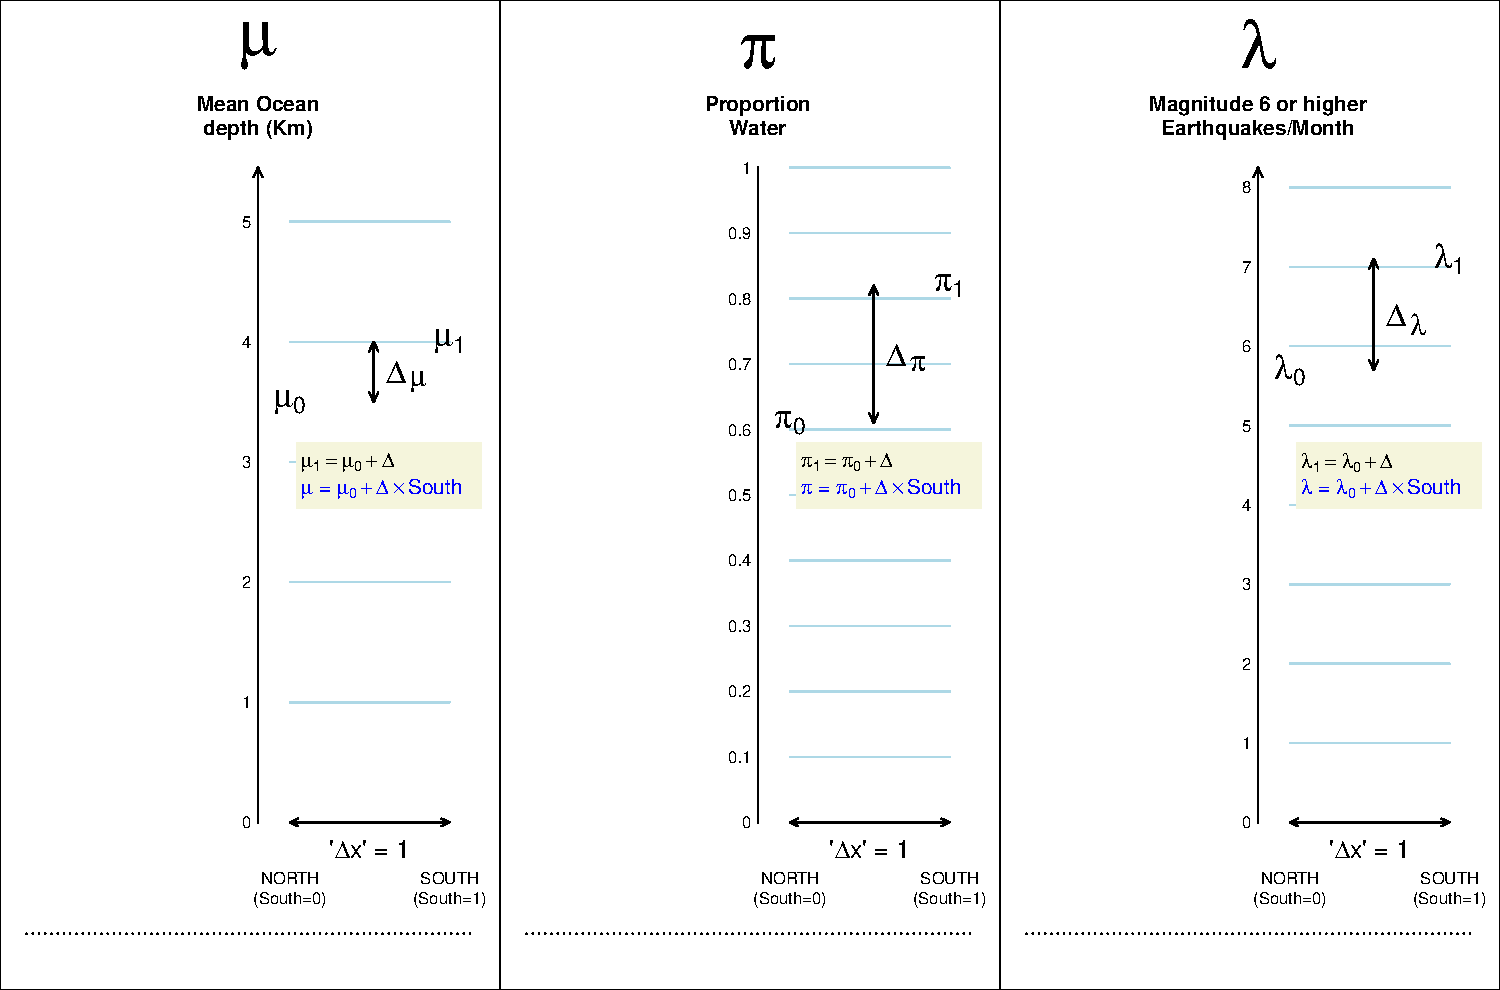
\includegraphics[width=4.9in,height=3.6in]{Fig12.pdf}
}
\end{frame}

\begin{frame}
\Wider[8em]{
	\centering
	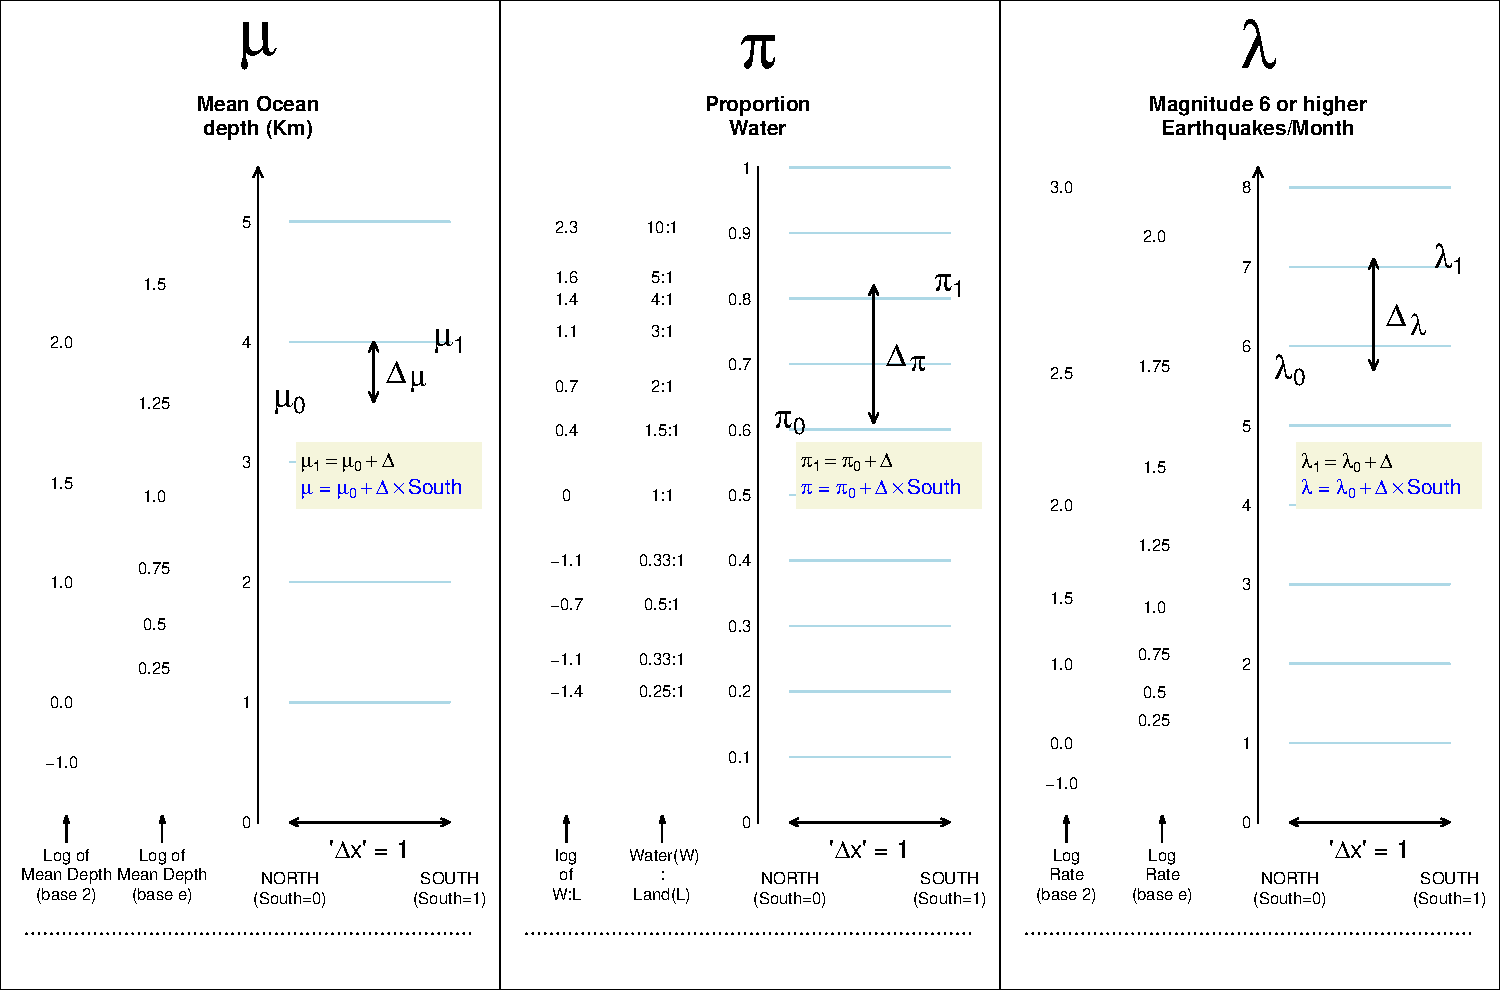
\includegraphics[width=4.9in,height=3.6in]{Fig13.pdf}
}
\end{frame}


\begin{frame}
\Wider[8em]{
	\centering
	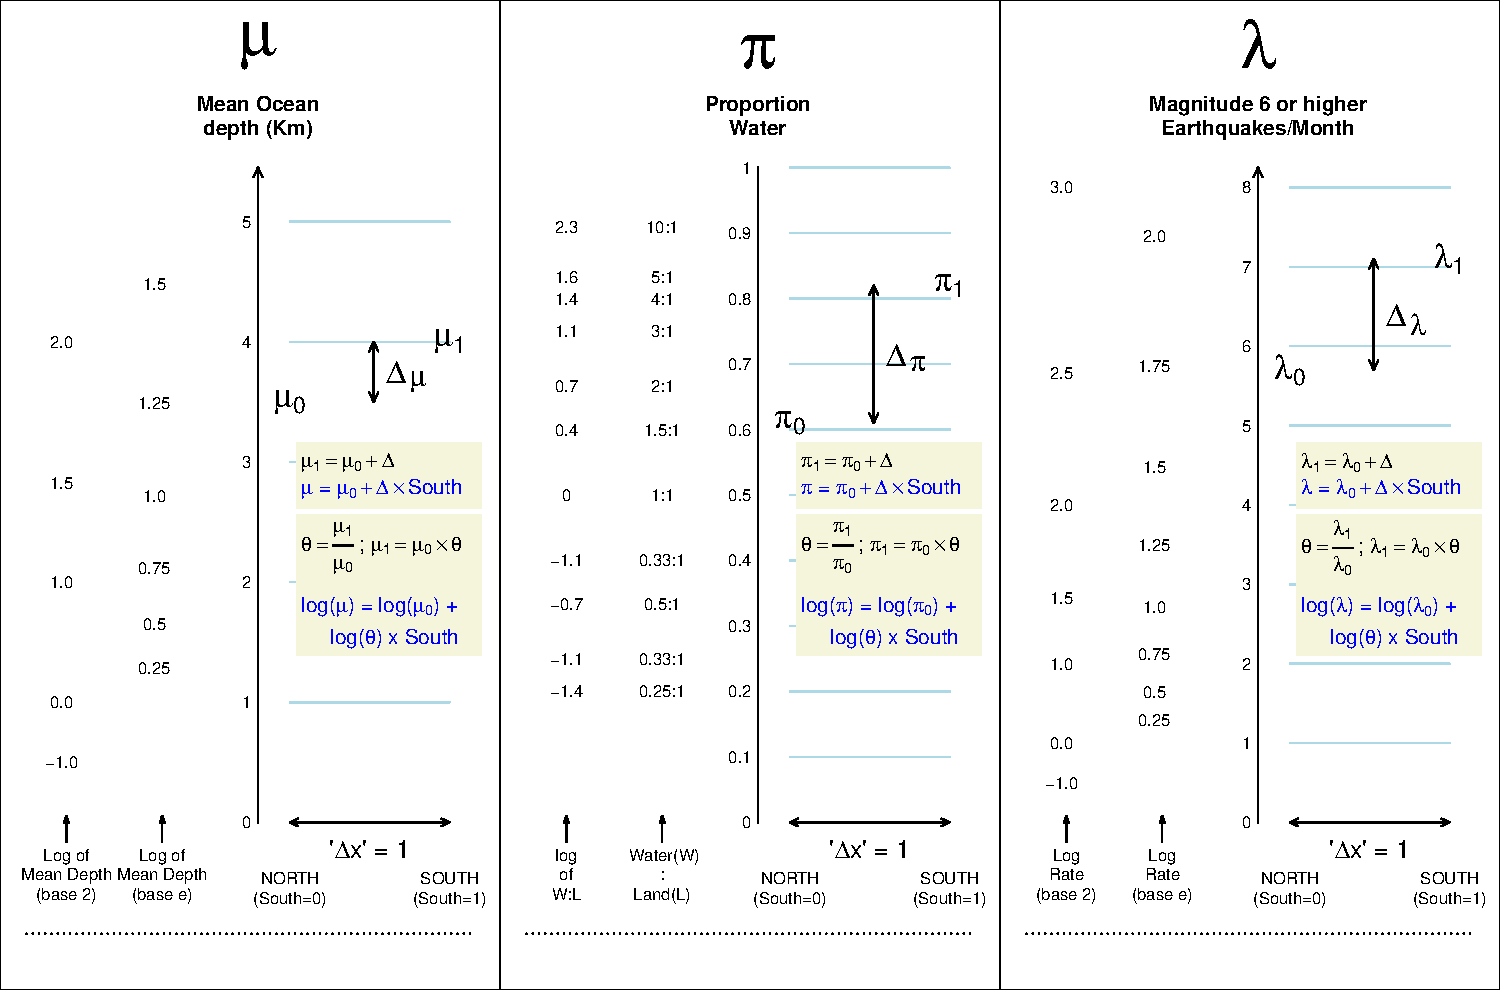
\includegraphics[width=4.9in,height=3.6in]{Fig14.pdf}
}
\end{frame}


\begin{frame}
\Wider[8em]{
	\centering
	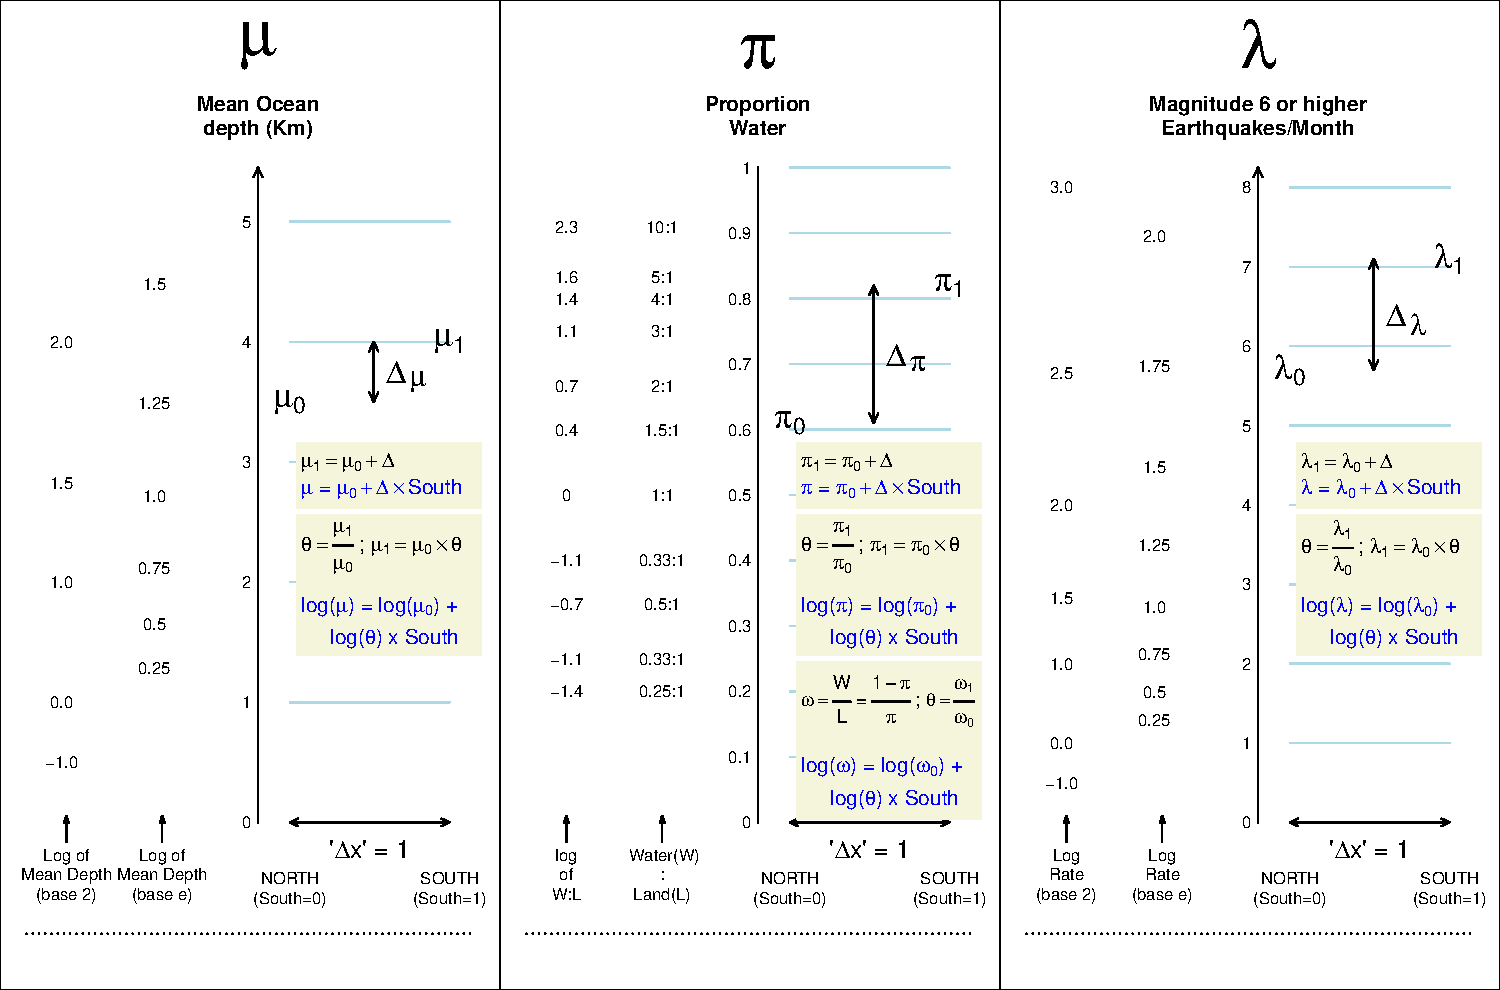
\includegraphics[width=4.9in,height=3.6in]{Fig15.pdf}
}
\end{frame}


\begin{frame}
\Wider[8em]{
	\centering
	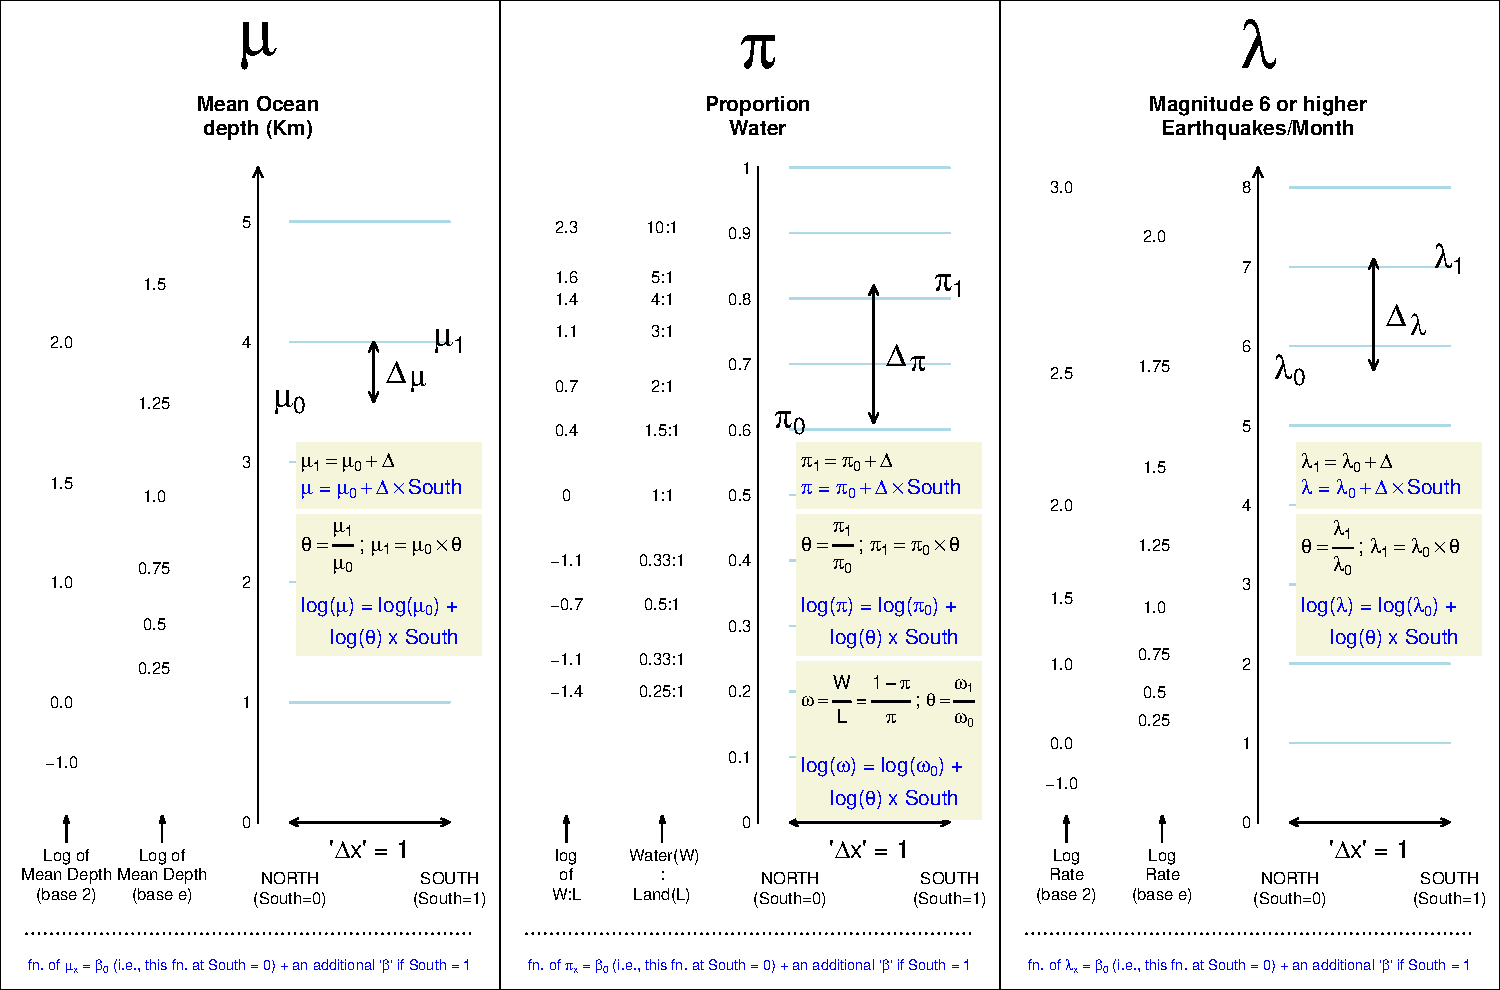
\includegraphics[width=4.9in,height=3.6in]{Fig16.pdf}
}
\end{frame}


\section{Fitting the regression equation with our sample data}



\begin{frame}[fragile]{Depths of the ocean: North vs. South Hemisphere}

\begin{knitrout}\tiny
\definecolor{shadecolor}{rgb}{0.969, 0.969, 0.969}\color{fgcolor}
\begin{alltt}
\hlcom{# load function to get depths}
\hlkwd{source}\hlstd{(}\hlstr{"https://github.com/sahirbhatnagar/EPIB607/raw/master/
exercises/water/automate_water_task.R"}\hlstd{)}

\hlcom{# get 1000 depths}
\hlkwd{set.seed}\hlstd{(}\hlnum{222333444}\hlstd{)}
\hlstd{depths} \hlkwb{<-} \hlkwd{automate_water_task}\hlstd{(}\hlkwc{index} \hlstd{=} \hlkwd{sample}\hlstd{(}\hlnum{1}\hlopt{:}\hlnum{50000}\hlstd{,} \hlnum{1000}\hlstd{),}
        \hlkwc{student_id} \hlstd{=} \hlnum{222333444}\hlstd{,} \hlkwc{type} \hlstd{=} \hlstr{"depth"}\hlstd{)}

\hlcom{# separate by north and south hemisphere}
\hlstd{depths_north} \hlkwb{<-} \hlstd{depths[}\hlkwd{which}\hlstd{(depths}\hlopt{$}\hlstd{lat}\hlopt{>}\hlnum{0}\hlstd{),]}
\hlstd{depths_south} \hlkwb{<-} \hlstd{depths[}\hlkwd{which}\hlstd{(depths}\hlopt{$}\hlstd{lat}\hlopt{<}\hlnum{0}\hlstd{),]}

\hlcom{# restrict sample to 200 (at random)}
\hlstd{depths_north} \hlkwb{<-} \hlstd{depths_north[}\hlkwd{sample}\hlstd{(}\hlnum{1}\hlopt{:}\hlkwd{nrow}\hlstd{(depths_north),} \hlnum{200}\hlstd{), ]}
\hlstd{depths_south} \hlkwb{<-} \hlstd{depths_south[}\hlkwd{sample}\hlstd{(}\hlnum{1}\hlopt{:}\hlkwd{nrow}\hlstd{(depths_south),} \hlnum{200}\hlstd{), ]}

\hlcom{# add indicator variable}
\hlstd{depths_north}\hlopt{$}\hlstd{South} \hlkwb{<-} \hlnum{0}
\hlstd{depths_south}\hlopt{$}\hlstd{South} \hlkwb{<-} \hlnum{1}

\hlcom{# combine data}
\hlstd{depths} \hlkwb{<-} \hlkwd{rbind}\hlstd{(depths_north, depths_south)}
\hlkwd{head}\hlstd{(depths)}

\hlcom{# calculate mean and sd by hemisphere}
\hlstd{means} \hlkwb{<-} \hlkwd{aggregate}\hlstd{(}\hlkwc{x} \hlstd{= depths,} \hlkwc{by} \hlstd{=} \hlkwd{list}\hlstd{(depths}\hlopt{$}\hlstd{South),} \hlkwc{FUN} \hlstd{=} \hlstr{"mean"}\hlstd{)}\hlopt{$}\hlstd{alt}
\hlstd{sds} \hlkwb{<-} \hlkwd{aggregate}\hlstd{(}\hlkwc{x} \hlstd{= depths,} \hlkwc{by} \hlstd{=} \hlkwd{list}\hlstd{(depths}\hlopt{$}\hlstd{South),} \hlkwc{FUN} \hlstd{=} \hlstr{"sd"}\hlstd{)}\hlopt{$}\hlstd{alt}
\end{alltt}

\end{knitrout}


\end{frame}


\begin{frame}[fragile]{Depths of the ocean: North vs. South Hemisphere}

\begin{knitrout}\tiny
\definecolor{shadecolor}{rgb}{0.969, 0.969, 0.969}\color{fgcolor}

{\centering 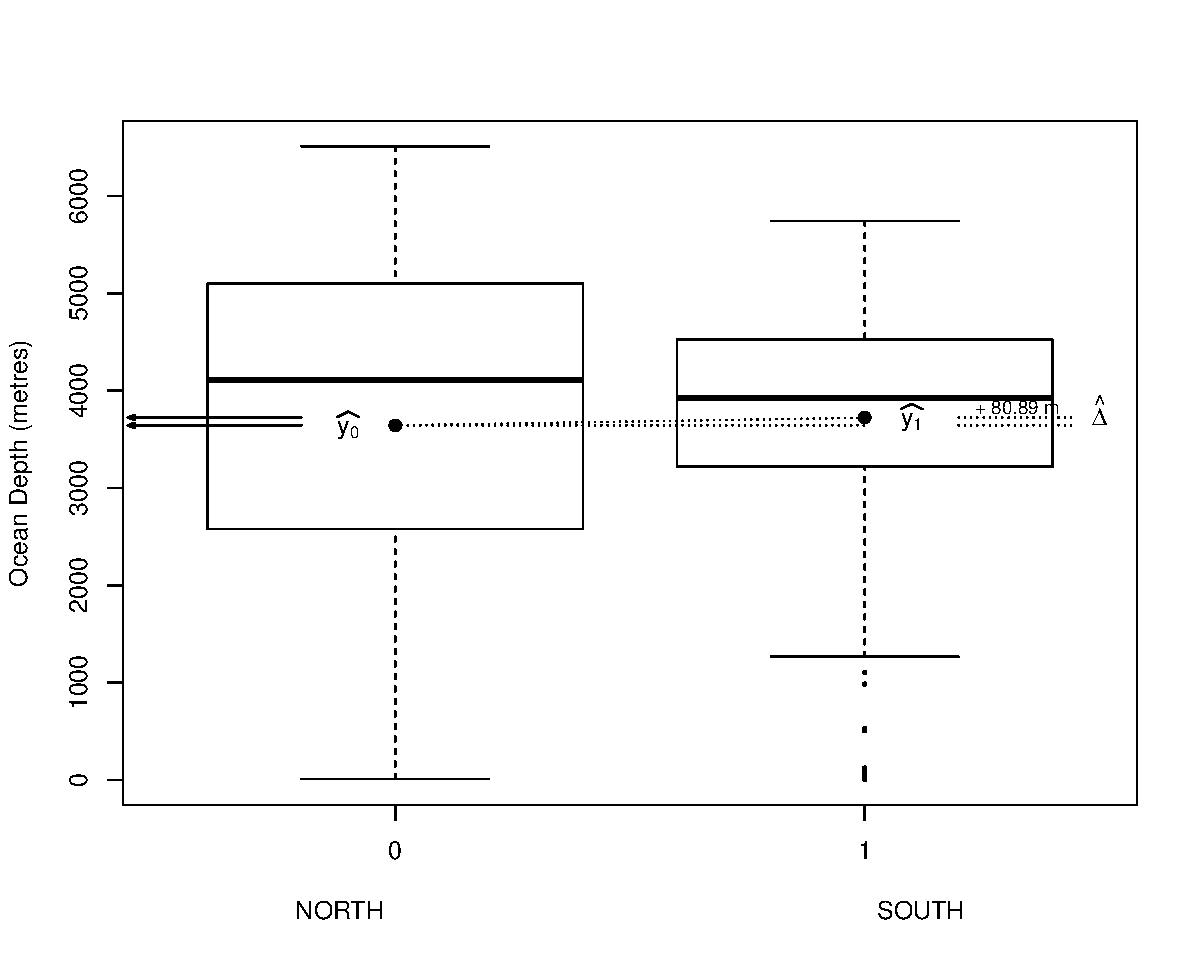
\includegraphics[width=1\linewidth]{figure/unnamed-chunk-2-1} 

}



\end{knitrout}


\end{frame}



\begin{frame}[fragile]{Standard error of the mean difference}

To perform inference we first need to calculate the SE of the mean difference given by:

\begin{equation}
SE_{\bar{y_1} - \bar{y_0}} = \sqrt{\frac{s_0^2}{n_0} + \frac{s_1^2}{n_1}}
\end{equation}

\pause 

\begin{knitrout}\scriptsize
\definecolor{shadecolor}{rgb}{0.969, 0.969, 0.969}\color{fgcolor}
\begin{alltt}
\hlstd{n0} \hlkwb{<-} \hlkwd{nrow}\hlstd{(depths_north)}
\hlstd{n1} \hlkwb{<-} \hlkwd{nrow}\hlstd{(depths_south)}

\hlstd{mean0} \hlkwb{<-} \hlkwd{mean}\hlstd{(depths_north}\hlopt{$}\hlstd{alt)}
\hlstd{mean1} \hlkwb{<-} \hlkwd{mean}\hlstd{(depths_south}\hlopt{$}\hlstd{alt)}

\hlstd{var0} \hlkwb{<-} \hlkwd{var}\hlstd{(depths_north}\hlopt{$}\hlstd{alt)}
\hlstd{var1} \hlkwb{<-} \hlkwd{var}\hlstd{(depths_south}\hlopt{$}\hlstd{alt)}

\hlstd{(SEM} \hlkwb{<-} \hlkwd{sqrt}\hlstd{(var0}\hlopt{/}\hlstd{n0} \hlopt{+} \hlstd{var1}\hlopt{/}\hlstd{n1))}
\end{alltt}
\begin{verbatim}
## [1] 157.565
\end{verbatim}

\end{knitrout}


\end{frame}



\begin{frame}[fragile]{95\% Confidence Interval for the Mean Difference}

We can then calculate a 95\% CI for the mean difference given by:

\begin{equation}
(\bar{y_1} - \bar{y_0}) \pm t^\star_{(n_0 + n_1 - 2)} \times SE_{\bar{y_1} - \bar{y_0}}
\end{equation}

\pause 

\begin{knitrout}\scriptsize
\definecolor{shadecolor}{rgb}{0.969, 0.969, 0.969}\color{fgcolor}
\begin{alltt}
\hlcom{# assuming equal variances}
\hlstd{(mean1} \hlopt{-} \hlstd{mean0)} \hlopt{+} \hlkwd{qt}\hlstd{(}\hlkwd{c}\hlstd{(}\hlnum{0.025}\hlstd{,} \hlnum{0.975}\hlstd{),} \hlkwc{df} \hlstd{= n0} \hlopt{+} \hlstd{n1} \hlopt{-} \hlnum{2}\hlstd{)} \hlopt{*} \hlstd{SEM}
\end{alltt}
\begin{verbatim}
## [1] -228.8787  390.6487
\end{verbatim}
\begin{alltt}
\hlcom{# similar to z interval}
\hlkwd{qnorm}\hlstd{(}\hlkwd{c}\hlstd{(}\hlnum{0.025}\hlstd{,} \hlnum{0.975}\hlstd{),} \hlkwc{mean} \hlstd{= mean1} \hlopt{-} \hlstd{mean0,} \hlkwc{sd} \hlstd{= SEM)}
\end{alltt}
\begin{verbatim}
## [1] -227.9367  389.7067
\end{verbatim}

\end{knitrout}


\end{frame}


\begin{frame}[fragile]{Parameter contrasts with regression}

Using the \texttt{lm} function in \texttt{R}:


\begin{knitrout}\scriptsize
\definecolor{shadecolor}{rgb}{0.969, 0.969, 0.969}\color{fgcolor}
\begin{alltt}
\hlcom{# regression. lm assumes equal variances}
\hlstd{fit} \hlkwb{<-} \hlkwd{lm}\hlstd{(alt} \hlopt{~} \hlstd{South,} \hlkwc{data} \hlstd{= depths)}
\hlkwd{summary}\hlstd{(fit)}
\end{alltt}
\begin{verbatim}
## 
## Call:
## lm(formula = alt ~ South, data = depths)
## 
## Residuals:
##     Min      1Q  Median      3Q     Max 
## -3722.0  -608.5   401.5  1200.4  2867.9 
## 
## Coefficients:
##             Estimate Std. Error t value Pr(>|t|)    
## (Intercept)  3643.08     111.42  32.698   <2e-16 ***
## South          80.88     157.56   0.513    0.608    
## ---
## Signif. codes:  0 '***' 0.001 '**' 0.01 '*' 0.05 '.' 0.1 ' ' 1
## 
## Residual standard error: 1576 on 398 degrees of freedom
## Multiple R-squared:  0.0006617,	Adjusted R-squared:  -0.001849 
## F-statistic: 0.2635 on 1 and 398 DF,  p-value: 0.608
\end{verbatim}

\end{knitrout}


\end{frame}


\begin{frame}[fragile]{Confidence interval from regression fit}

\begin{knitrout}\scriptsize
\definecolor{shadecolor}{rgb}{0.969, 0.969, 0.969}\color{fgcolor}
\begin{alltt}
\hlkwd{confint}\hlstd{(fit)}
\end{alltt}
\begin{verbatim}
##                 2.5 %    97.5 %
## (Intercept) 3424.0440 3862.1160
## South       -228.8787  390.6487
\end{verbatim}

\end{knitrout}


\end{frame}



\begin{frame}[fragile]{Unequal variances using \texttt{stats::t.test}}

\texttt{stats::t.test} assumes unequal variances by default:


\begin{knitrout}\scriptsize
\definecolor{shadecolor}{rgb}{0.969, 0.969, 0.969}\color{fgcolor}
\begin{alltt}
\hlkwd{t.test}\hlstd{(alt} \hlopt{~} \hlstd{South,} \hlkwc{data} \hlstd{= depths,} \hlkwc{var.equal} \hlstd{=} \hlnum{FALSE}\hlstd{)}
\end{alltt}
\begin{verbatim}
## 
## 	Welch Two Sample t-test
## 
## data:  alt by South
## t = -0.51334, df = 349.62, p-value = 0.608
## alternative hypothesis: true difference in means is not equal to 0
## 95 percent confidence interval:
##  -390.7795  229.0095
## sample estimates:
## mean in group 0 mean in group 1 
##        3643.080        3723.965
\end{verbatim}
\begin{alltt}
\hlstd{(mean0} \hlopt{-} \hlstd{mean1)} \hlopt{+} \hlkwd{qt}\hlstd{(}\hlkwd{c}\hlstd{(}\hlnum{0.025}\hlstd{,} \hlnum{0.975}\hlstd{),} \hlkwc{df} \hlstd{=} \hlnum{349.61783}\hlstd{)} \hlopt{*} \hlstd{SEM}
\end{alltt}
\begin{verbatim}
## [1] -390.7795  229.0095
\end{verbatim}

\end{knitrout}


\end{frame}



\begin{frame}[fragile]{Equal variances using \texttt{stats::t.test}}

We can specify equal variance assumption in \texttt{stats::t.test}:

\begin{knitrout}\scriptsize
\definecolor{shadecolor}{rgb}{0.969, 0.969, 0.969}\color{fgcolor}
\begin{alltt}
\hlkwd{t.test}\hlstd{(alt} \hlopt{~} \hlstd{South,} \hlkwc{data} \hlstd{= depths,} \hlkwc{var.equal} \hlstd{=} \hlnum{TRUE}\hlstd{)}
\end{alltt}
\begin{verbatim}
## 
## 	Two Sample t-test
## 
## data:  alt by South
## t = -0.51334, df = 398, p-value = 0.608
## alternative hypothesis: true difference in means is not equal to 0
## 95 percent confidence interval:
##  -390.6487  228.8787
## sample estimates:
## mean in group 0 mean in group 1 
##        3643.080        3723.965
\end{verbatim}
\begin{alltt}
\hlstd{(mean0} \hlopt{-} \hlstd{mean1)} \hlopt{+} \hlkwd{qt}\hlstd{(}\hlkwd{c}\hlstd{(}\hlnum{0.025}\hlstd{,} \hlnum{0.975}\hlstd{),} \hlkwc{df} \hlstd{= n0} \hlopt{+} \hlstd{n1} \hlopt{-} \hlnum{2}\hlstd{)} \hlopt{*} \hlstd{SEM}
\end{alltt}
\begin{verbatim}
## [1] -390.6487  228.8787
\end{verbatim}

\end{knitrout}


\end{frame}


\end{document}




